\documentclass{hwset}

% info for header block in upper right hand corner
\name{Erich L Foster}
\class{Calculus I}
\duedate{Due: 24 January 2011}
\assignment{Homework 1}

\begin{document}
\begin{problem}[1.] Suppose $f$ is defined on $[-1,3]$ and satisfies:
	\begin{equation*}
		f(x)=\begin{cases} x, &  -1 \leq x < 0 \\
			-\frac{1}{2}x^{2}, & 0 \leq x < 1 \\
    	\sqrt{1-(x-2)^{2}}, & 1 \leq x \leq 3, x \ne 2 \\
    	0, & x = 2
		\end{cases}
	\end{equation*}
	\be
		\item Sketch the graph of the function given above.
		\item Does $\lim_{x\to 2}f(x)$ exist? Justify your answer.
		\item Does $\lim_{x\to 1}f(x)$ exist? Justify your answer.
		\item Does $\lim_{x\to 4}f(x)$ exist? Justify your answer.
	\ee
\end{problem}

\be
	\item \begin{solution}
	\begin{figure}[H]
	\begin{center}
		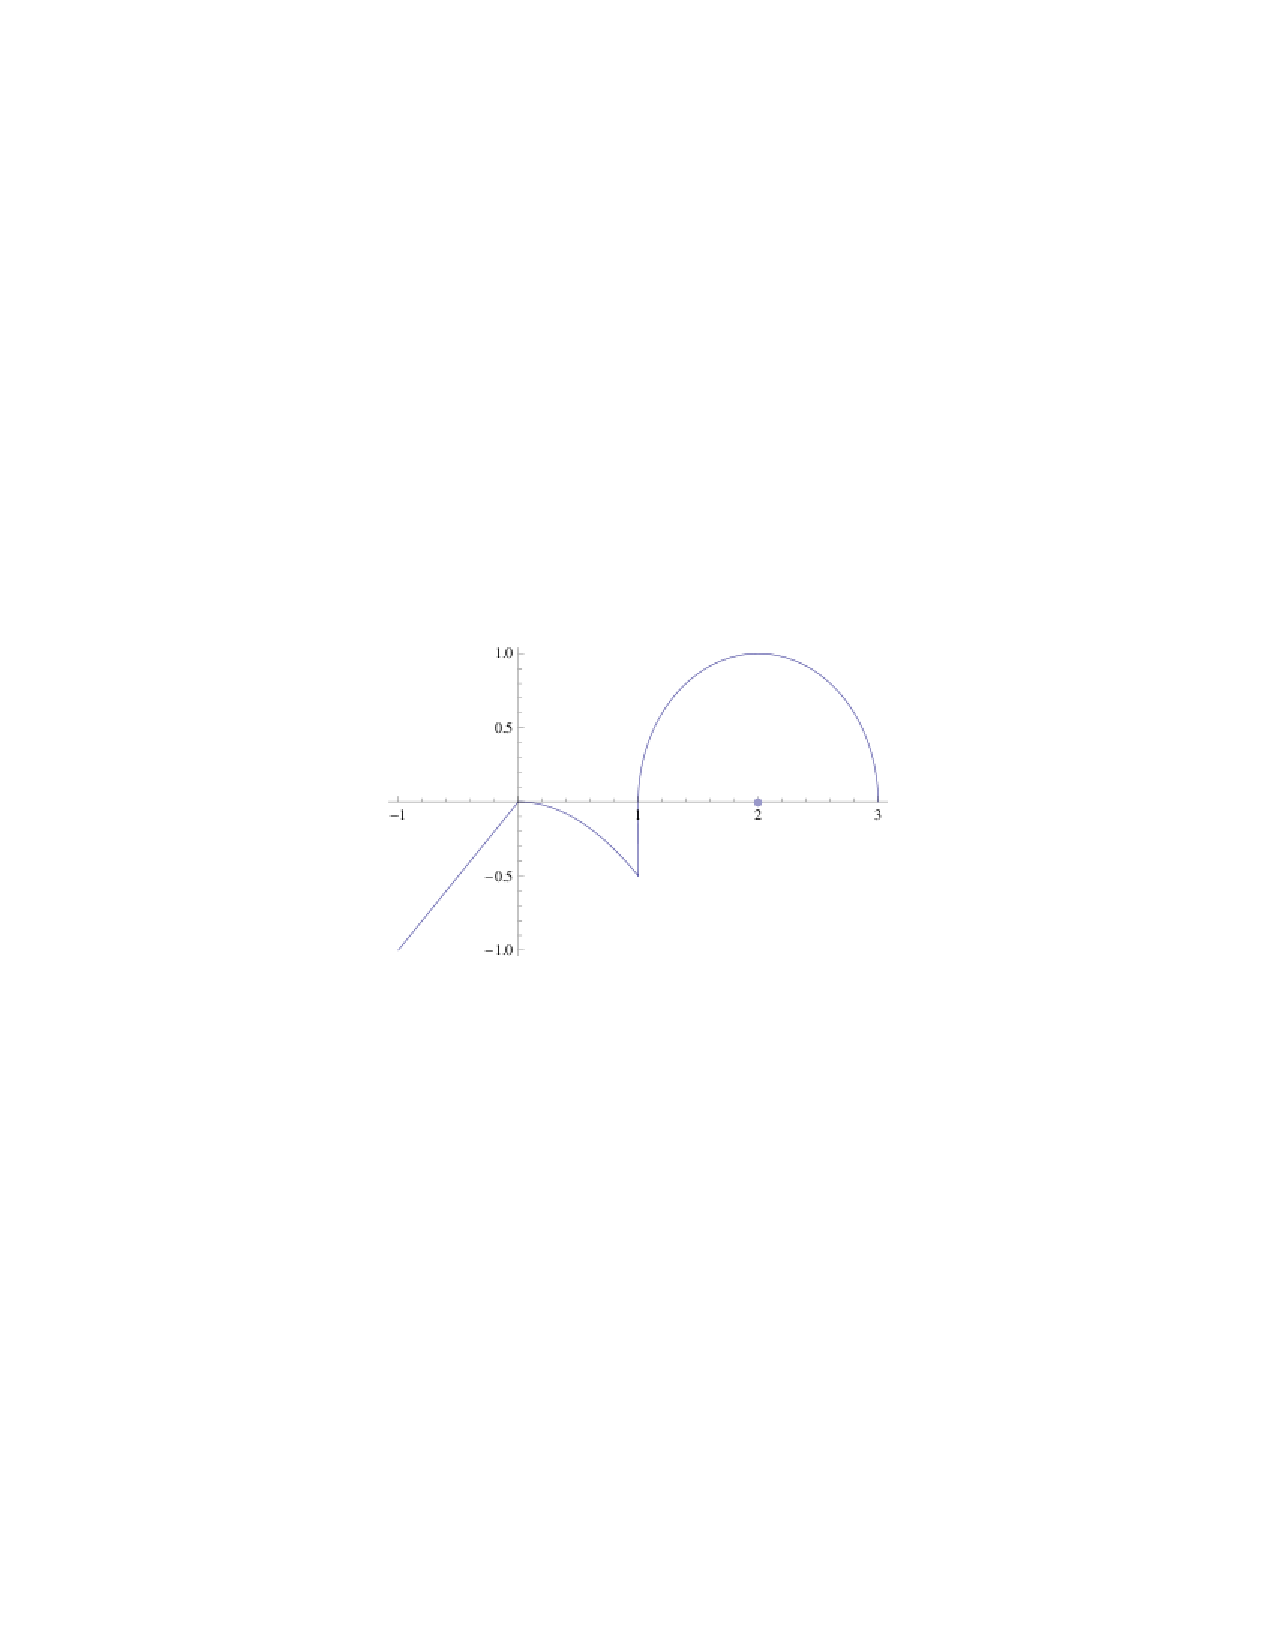
\includegraphics[trim=200 300 280 290]{HW1_1.pdf} \\
	\end{center}
	\end{figure}
	\end{solution}
	\item \begin{solution}
		Yes, the limit exists, because the function approaches the same value from
		the left and from the right, i.e 1.
	\end{solution}
	\item \begin{solution}
		No, the limit doesn't exist because the function approaches two different
		values from either side, i.e $-\frac{1}{2}$ from the left and $0$ from the
		right.
	\end{solution}
	\item \begin{solution}
		No, the limit doesn't exist, since the function is not defined for values of
		$x$ outside of $[-1, 3].$
	\end{solution}
\ee

\begin{problem}[2.]
	\be
		\item Suppose that a function $f(x)$ is defined for all $x\in[-2,2]$. Can
		anything be said about the existence of $\lim_{x\to 0}f(x)$? Give reasons
		for your answer.
		\item Suppose that $g$ is a function defined for all $x$. If $g(1)=5$, must
		$\lim_{x\to1}g(x)$ exist? If it does, then must $ \lim_{x\to1}g(x)=5$? Can
		we conclude anything about $\lim_{x\to1}g(x)$? Explain!
	\ee
\end{problem}

\be
	\item \begin{solution}
		No, we cannot say anything about the existence of $\lim_{x \to 0} f(x)$,
		because we don't know the behavior of the function near $x=0$.
	\end{solution}
	\item \begin{solution}
		No, the limit does not need to exists, since the value of the function could
		approach one value from the left and a different value from the right. If
		the limit does exist it does not have to be equal to $g(1)$, since the
		function could be piecewise, e.g.
		\begin{equation*}
			g(x) = \begin{cases}
				x^2 & x \ne 1 \\
				5 & x = 1
			\end{cases}
		\end{equation*}
		The $lim_{x \to 1} g(x) = 1 \ne g(1) = 5$. We cannot conclude anything about
		$\lim_{x\to 0} g(x)$, since we do not have enough information about the
		function.
	\end{solution}
\ee

\begin{problem}[3.] Find the following limits.
	\be
		\item $\lim_{h\to 0}\dfrac{\sqrt{5h+4}-2}{h}$
		\item $\lim_{x\to -2}\dfrac{x+2}{\sqrt{x^2+5}-3}$
		\item $\lim_{t\to 0}\dfrac{1+t+\sin(t)}{3\cos(t)}$
		\item $\lim_{u\to 1}\dfrac{u^{6}-1}{u^{4}-1}$
	\ee
\end{problem}

\be
	\item \begin{solution}
		\begin{align*}
			\lim_{h\to 0}\dfrac{\sqrt{5h+4}-2}{h} 
				&= \lim_{h\to 0}\dfrac{\sqrt{5h+4}-2}{h} \cdot \dfrac{\sqrt{5h + 4} +
					2}{\sqrt{5h + 4} + 2} \\ 
			&= \lim_{h\to 0} \dfrac{5h + 4 - 4}{h\cdot \sqrt{5h+4} + 2} \\
			&= \lim_{h\to 0} \dfrac{5h}{h\cdot \sqrt{5h+4} + 2} \\
			&= \lim_{h\to 0} \dfrac{5}{\sqrt{5h+4} + 2} \\
			&= \dfrac{5}{\lim_{h\to 0} \sqrt{5h+4} + 2} \\
			&= \dfrac{5}{\sqrt{\lim_{h\to 0}\left(5h+4\right)} + 2} \\
			&= \dfrac{5}{\sqrt{\lim_{h\to 0}\left(5h\right)+4} + 2} \\
			&= \dfrac{5}{\sqrt{4} + 2} \\
			&= \boxed{\dfrac{5}{4}.}
		\end{align*}
	\end{solution}
	\item \begin{solution}
		\begin{align*}
		\lim_{x\to -2}\dfrac{x+2}{\sqrt{x^2+5}-3} 
			&= \lim_{x\to -2}\dfrac{x+2}{\sqrt{x^2+5}-3}
				\dfrac{\sqrt{x^2+5}+3}{\sqrt{x^2+5}+3} \\
		&= \lim_{x\to -2}\dfrac{(x+2)(\sqrt{x^2+5}+3)}{x^2+5-9} \\
		&= \lim_{x\to -2}\dfrac{(x+2)(\sqrt{x^2+5}+3)}{x^2-4} \\
		&= \lim_{x\to -2}\dfrac{(x+2)(\sqrt{x^2+5}+3)}{(x-2)(x+2)} \\
		&= \dfrac{\lim_{x\to -2}(\sqrt{x^2+5}+3)}{\lim_{x\to -2}(x-2)} \\
		&= \dfrac{\sqrt{(-2)^2+5}+3)}{-2-2} \\
		&= -\dfrac{\sqrt{9}+3)}{4} \\
		&= -\dfrac{6}{4} \\
		&= \boxed{-\frac{3}{2}.}
		\end{align*}
	\end{solution}
	\item \begin{solution}
		\begin{align*}
			\lim_{t\to 0}\dfrac{1+t+\sin(t)}{3\cos(t)} 
				&= \dfrac{\lim_{t\to 0}\left(1+t+\sin(t)\right)}{\lim_{t\to 0} 3\cos(t)} \\
			&= \dfrac{1+0+\sin(0)}{3\cos(0)} \\
			&= \boxed{\dfrac{1}{3}.}
		\end{align*}
	\end{solution}
	\item \begin{solution}
		\begin{align*}
			\lim_{u\to 1}\dfrac{u^{6}-1}{u^{4}-1}
				&= \lim_{u\to 1}\dfrac{(u^{3}-1)(u^{3}+1)}{(u^{2}-1)(u^2+1)} \\
			&= \lim_{u\to 1}\dfrac{(u^{3}-1)(u^{3}+1)}{(u^{2}-1)(u^2+1)} \\
			&= \lim_{u\to 1}\dfrac{(u-1)(u^{2}+u+1)(u^{3}+1)}{(u+1)(u-1)(u^2+1)} \\
			&= \lim_{u\to 1}\dfrac{(u^{2}+u+1)(u^{3}+1)}{(u+1)(u^2+1)} \\
			&= \dfrac{(1^{2}+1+1)(1^{3}+1)}{(1+1)(1^2+1)} \\
			&= \dfrac{3\cdot 2}{2 \cdot 2} \\
			&= \dfrac{6}{4} \\
			&= \boxed{\dfrac{3}{2}.}
		\end{align*}
	\end{solution}
\ee

\begin{problem}[4.] Use Sandwich Theorem and limit laws to show that
	\be
		\item $\lim_{t\to 0}t^{2}\cos(20\pi t)=0$
		\item $\lim_{x\to 0}\sqrt{x^{3}+x^{2}}\sin({\frac{\pi}{x}})=0$
		\item $\lim_{h\to 0}\Big(h^{2}\cos(\frac{2}{h})+1\Big)\Big(h^{2}\cos(\frac{2}{h})-1\Big)=-1$
		\item $\lim_{u\to 0}u^{2}4^{\sin(\frac{\pi}{u})}=0$
	\ee
\end{problem}

\be
	\item \begin{solution}
		\begin{equation*}
			-1\le \cos(20\pi t) \le 1 \Rightarrow -t^2 \le t^{2}\cos(20\pi t) \le t^2.
		\end{equation*}
		\begin{align*}
			\lim_{t\to 0} -t^2 &= 0 \\
			\lim_{t\to 0} t^2 &= 0 
		\end{align*}
		Thus, by the Squeeze Theorem we see that $\lim_{t\to 0}t^{2}\cos(20\pi t)=0.$
	\end{solution}
	\item \begin{solution}
		\begin{equation*}
			-1\le \sin(\frac{\pi}{x}) \le 1 \Rightarrow -\sqrt{x^3 +x^2} \le \sqrt{x^3
			+ x^2} \sin(\frac{\pi}{x}) \le \sqrt{x^3 + x^2}.
		\end{equation*}
		\begin{align*}
			\lim_{x\to 0} -\sqrt{x^3+x^2} &= 0 \\
			\lim_{t\to 0} \sqrt{x^3+x^2} &= 0 
		\end{align*}
		Thus, by the Squeeze Theorem we see that $\lim_{x\to
		0}\sqrt{x^3+x^2}\sin(\frac{\pi}{x})=0.$
	\end{solution}
	\item \begin{solution}
		\begin{equation*}
			\left(h^2 \cos(\frac{2}{h} + 1\right)\left(h^2 \cos(\frac{2}{h} - 1\right)
				= h^4 \cos^2(\frac{2}{h} - 1
		\end{equation*}
		\begin{align*}
			&0 \le \cos^2(\frac{2}{h}) \le 1 \\
			&\Rightarrow 0 \le h^2\cos(\frac{2}{h})\le h^2 
			&\Rightarrow -1 \le h^2\cos(\frac{2}{h}) - 1 \le h^2 - 1
		\end{align*}
		\begin{align*}
			\lim_{x\to 0} - 1 &= -1 \\
			\lim_{x\to 0} h^2 - 1 &= -1 
		\end{align*}
		Thus, by the Squeeze Theorem we see that 
		$\lim_{h\to 0}\Big(h^{2}\cos(\frac{2}{h})+1\Big)\Big(h^{2}\cos(\frac{2}{h})-1\Big)=-1$
	\end{solution}
	\item \begin{solution}
		\begin{equation*}
			-1\le \sin(\frac{\pi}{u}) \le 1 \Rightarrow 4^{-1} u^2 \le u^2
			4^{\sin(\frac{\pi}{u}} \le 4 u^2.
		\end{equation*}
		\begin{align*}
			\lim_{u\to 0} 4^{-1} u^2 &= 0 \\
			\lim_{u\to 0} 4 u^2 &= 0 
		\end{align*}
		Thus, by the Squeeze Theorem we see that $\lim_{u\to
		0} u^2 4^{\sin(\frac{\pi}{u})}=0.$
	\end{solution}
\ee

\end{document}
